
%https://tex.stackexchange.com/questions/438530/drawing-a-rough-surface-with-tikz
\documentclass[tikz,border=5]{standalone}
\usetikzlibrary{decorations.pathmorphing}

\pgfdeclaredecoration{jiggly}{step}
{
	\state{step}[width=+\pgfdecorationsegmentlength]
	{\pgfmathsetmacro{\delta}{rand*\pgfdecorationsegmentamplitude}
		\pgfpathlineto{
			\pgfpointadd
			{\pgfpoint{\pgfdecorationsegmentlength}{0pt}}
			{\pgfpointpolar{90-\pgfdecoratedangle}
				{\delta}}
		}
	}
	\state{final}
	{
		\pgfpathlineto{\pgfpointdecoratedpathlast}
	}
}


\begin{document}
	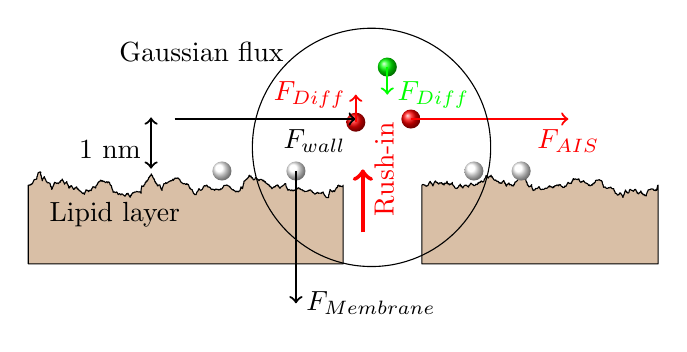
\begin{tikzpicture}[line join=round]
% left side of the channel		
		\draw[fill=orange!40!gray!50!white]
		{decorate[decoration={jiggly, segment length=0.25,amplitude=0.25}]
			{decorate[decoration={jiggly, segment length=1,amplitude=1}]
				{decorate[decoration={jiggly, segment length=4,amplitude=4}]     
					{(0,0) -- ++(4,0)}}}} -- ++(0,-10mm) -- ++(-4cm,0) -- cycle;
% right side of the channel
		\draw[fill=orange!40!gray!50!white]
{decorate[decoration={jiggly, segment length=0.25,amplitude=0.25}]
	{decorate[decoration={jiggly, segment length=1,amplitude=1}]
		{decorate[decoration={jiggly, segment length=4,amplitude=4}]     
			{(5,0) -- ++(3,0)}}}} -- ++(0,-10mm) -- ++(-3cm,0) -- cycle;
		
% Ions on the surface
 \shade[ball color=white] (3.40,0.18) circle (.8ex);
 \shade[ball color=white] (2.46,0.18) circle (.8ex);
 \shade[ball color=white] (5.66,0.18) circle (.8ex);
\shade[ball color=white] (6.26,0.18) circle (.8ex);
% Ions from the rush-in
 \shade[ball color=red] (4.16,0.80) circle (.8ex);
 \shade[ball color=red] (4.86,0.84) circle (.8ex);
% Kicked-out K+ ions
 \shade[ball color=green] (4.56,1.5) circle (.8ex);
 
 % Forces exerting on ions
         \draw[thick,->,color=black] (3.40,0.18)--(3.40,-1.5) node[right] {$F_{Membrane}$};
         \draw[thick,->,color=red, below] (4.86,0.84)--(6.86,0.84) node[below] {$F_{AIS}$};
         \draw[thick,->,color=black,left] (1.86,0.84)--(4.16,0.84) node[below left,color=black] {$F_{wall}$};
         % Diffusion forces
%         \draw[thick,->,color=green] [node] {$F_{Diff}$};
         \draw[thick,->,color=red] (4.16,0.8)--(4.16,1.15) node[left] {$F_{Diff}$};
         \draw[thick,->,color=green] (4.56,1.5)--(4.56,1.15) node[right] {$F_{Diff}$};
         % Rushin direction
		\draw[ultra thick,->,color=red, below]
		(4.25,-0.6)--(4.25,0.2) node[below,rotate=90] {Rush-in};
% Gaussian flux
 		 \draw[thin,color=black] (4.36,0.48) circle (10ex);
% 		 \draw[thick,color=black] (2.36,0.98) label{Gaussian flux};
 		\node[  label=Gaussian flux, above]  at (2.2,1.2) {};
 		 \node[  label=Lipid layer, above]  at (1.1,-0.9) {};
 		
 		% Approximate size
       \draw[thick,<->,color=black] (1.56,0.86)--(1.56,0.21) node[above left] {1 nm};
	\end{tikzpicture}
\end{document}

